\documentclass[12pt]{article}
\usepackage{mathpazo}
\usepackage{hyperref}
\usepackage{amsmath}
\usepackage{enumitem}
\usepackage{graphicx}
\usepackage{xcolor}
\usepackage{textcomp}
\usepackage{booktabs}
\usepackage{longtable}
\usepackage{soul}
\setuldepth{model}
\usepackage{everysel}
\usepackage{pgfplots}

% This is to fix full justification for \texttt{}. Credit:
% https://texblog.net/latex-archive/plaintex/full-justification-with-typewriter-font/
\ttfamily
\fontdimen2\font=0.4em% interword space
\fontdimen3\font=0.2em% interword stretch
\fontdimen4\font=0.1em% interword shrink
\fontdimen7\font=0.1em% extra space

% Credit: Stefan Kottwitz, https://latex.org/forum/viewtopic.php?t=13230
\newcommand*{\Biggg}[1]{\vcenter{\hbox{\scalebox{3}{\ensuremath#1}}}}
\newcommand*{\Bigggg}[1]{\vcenter{\hbox{\scalebox{8}{\ensuremath#1}}}}

\usepackage[top=2.54cm, bottom=2.54cm, left=2.54cm, right=2.54cm]{geometry}
\usepackage{tikz}
\usetikzlibrary{fit}
\usetikzlibrary{calc}
\usetikzlibrary{matrix}
\usetikzlibrary{calligraphy}
\usetikzlibrary{arrows.meta}
\usetikzlibrary{shapes.misc}
\usetikzlibrary{intersections}
\usetikzlibrary{shapes,arrows}
\usetikzlibrary{shapes.multipart}
\usetikzlibrary{shapes.geometric}
\usetikzlibrary{shadows,shadings}
\usetikzlibrary{tikzmark,positioning}
\usetikzlibrary{decorations.markings}
\usetikzlibrary{decorations.pathreplacing}

\tikzstyle{stochnode}=[black, draw=black, line width=1.5pt, shape=circle, fill=white, minimum size=8mm, inner sep=3pt]

\tikzstyle{detnode}=[black, draw=black, line width=1.5pt, densely dashed, shape=circle, fill=white, minimum size=8mm, inner sep=3pt]

\tikzstyle{constnode}=[black, draw=black, line width=1.5pt, shape=regular polygon, regular polygon sides=4, fill=white, minimum size=8mm, inner sep=1pt, align=center]

\tikzstyle{clampnode}=[black, draw=black, line width=1.5pt, shape=circle, fill=black!20!white, minimum size=8mm, inner sep=3pt]

\begin{document}
\frenchspacing

\begin{center}
{\Large \textbf{Lab 8. Estimating time trees}} \\[0.5cm]
{\large Due Wednesday, November 30, 2022 at 3 pm}
\end{center}

\vspace{1cm}

\noindent So far, we have focused on estimating \textit{cladograms} (with meaningless branch lengths) or \textit{phylograms} (with branch lengths in units of change per character). Today, we are going to infer \textit{chronograms}, or time trees: phylogenetic trees with branch lengths in units of calendar time. We are going to build on what we've learned in the last two labs, and do it using RevBayes: it's going to be much easier now that you're familiar with the program! \\

\hrule

\section*{Theory}

In Lab 4, we compared the fit of different cladograms to the stratigraphic record, and suggested that we could use this criterion to decide between different most parsimonious trees (which, by definition, are all equally ``good'' based on parsimony alone). In doing so, we briefly mentioned the fact that there are more sophisticated methods that can leverage stratigraphic age information not just to decide between competing topologies, but to infer them in the first place. It is these methods that we are going to explore today. \\

\noindent By now, we are quite used to phylograms, whose branch lengths confound \textit{rate} and \textit{time}. In a phylogram, the length of a branch expresses the amount of character change that has been accumulated along it, but there is no way to determine whether this amount is due to slow change happening over a long period of time, or rapid change happening over a short period of time. In statistical parlance, we would say that these quantities are \textit{not identifiable} from character data alone. This is a pretty intuitive idea: if I tell you I live two miles from my workplace, and ask you how long you think it takes me to get there, you'll likely find that information insufficient. That's because here, too, distance is the product of rate and time. On the other hand, if I give you an additional piece of data -- e.g., that I drive to work during rush hour -- you'll be able to come up with a decent estimate, since you can now disentangle the two factors. It works just the same with phylogenies: \\

\begin{center}
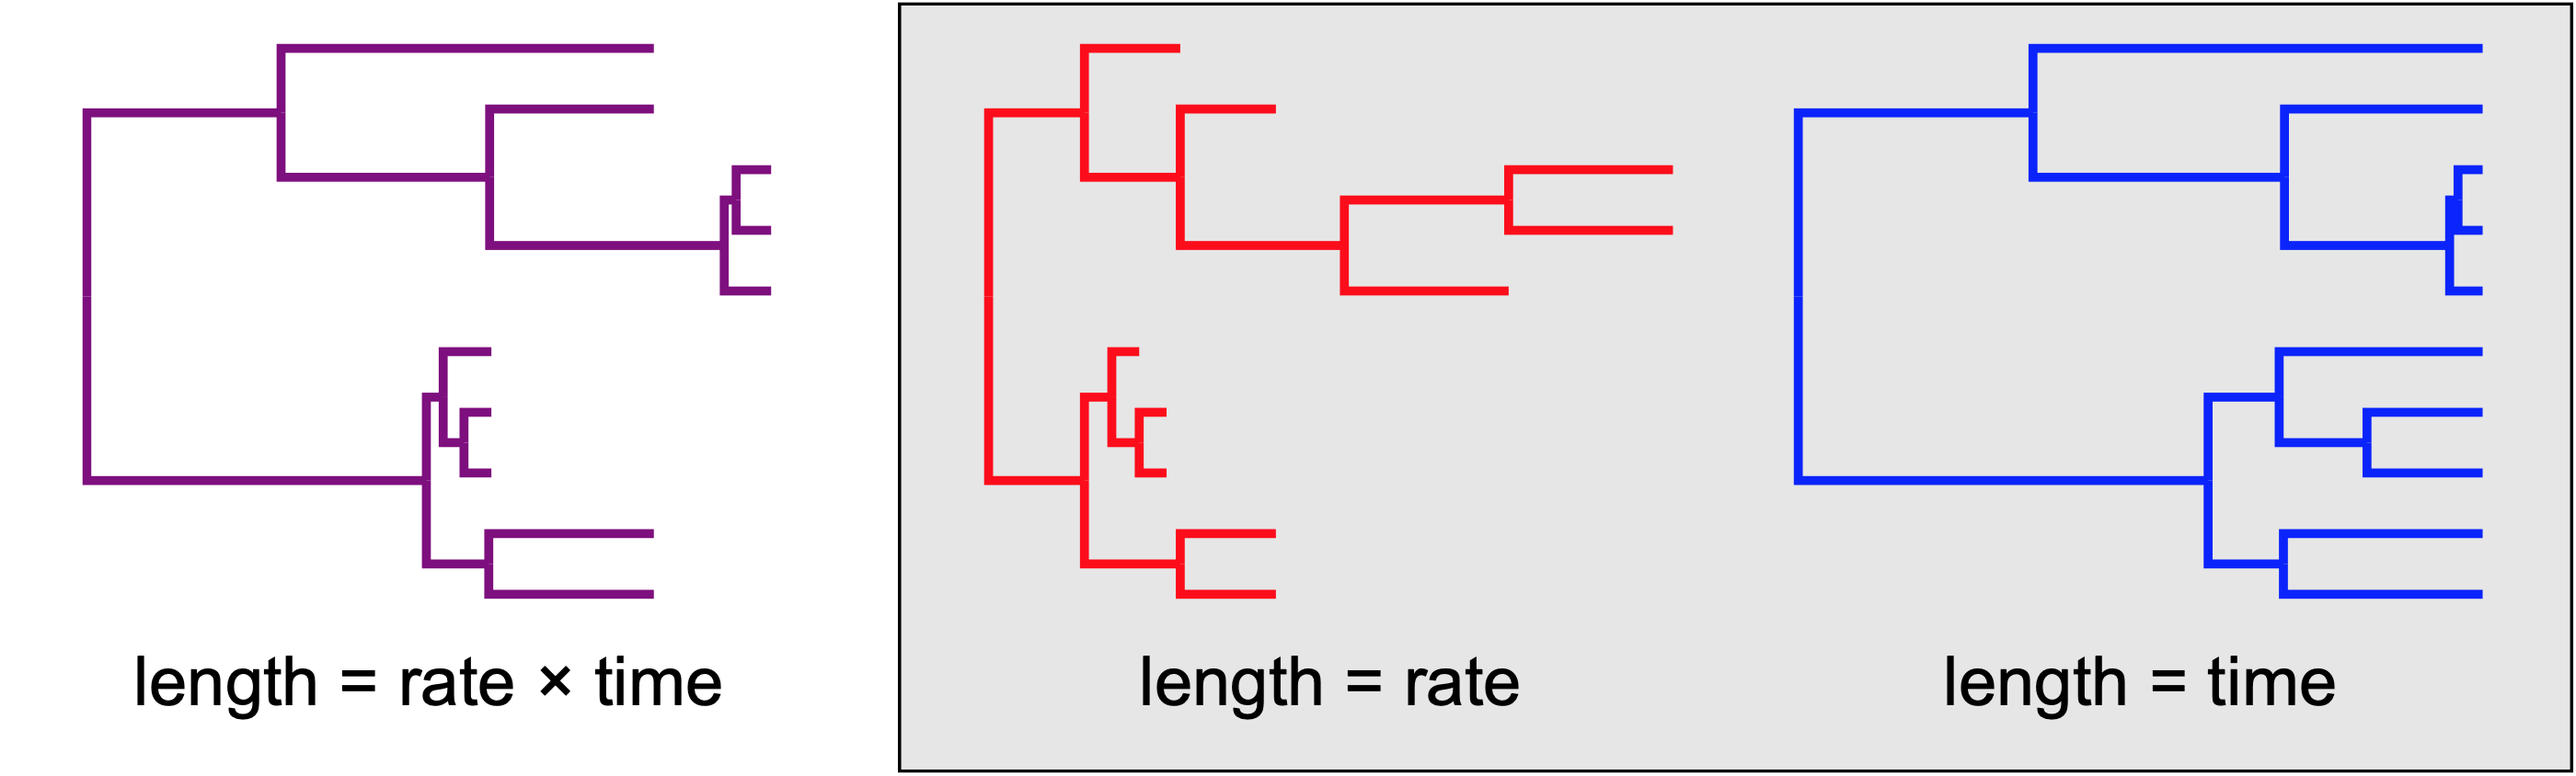
\includegraphics[width=\textwidth]{rate-vs-time.png} \\
\textcolor{gray!50!black}{\footnotesize Image credit: Tracy A. Heath, Iowa State University}
\end{center}

\noindent The earliest attempt to tease apart the relative contributions of rate and time to the total amount of character change is known as the \textit{strict clock} hypothesis, and dates back to the early 1960s, when the biochemists \'{E}mile Zuckerkandl and Linus Pauling noticed that the number of changes between the hemoglobin proteins of different species of mammals appeared to be proportional to the time elapsed since their last common ancestor, according to paleontological estimates. If that were the case, we would just have to determine the exact constant of proportionality, or the slope of the line when the amount of change is plotted against age. This is exactly what many researchers attempted to do: they would take a fossil they believed to be close in time to a particular divergence, and use it to ``calibrate the clock'' in order to convert branch lengths from units of substitutions per character into units of time. If, for example, two taxa differed in 5 out of 100 characters, and fossil evidence suggested their evolutionary lineages diverged 20 million years ago, we would conclude that the rate of evolution equals $(5/100)/(2 \times 20)$ = 0.00125 changes per character per million years. Once we've obtained this proportionality constant, converting the remaining branches into units of time is a matter of simple cross-multiplication. \\

\noindent It would be nice if things were this simple, wouldn't it? No such luck, unfortunately. It became clear quite early on that certain lineages evolve much faster than others, which really throws a wrench into the strict clock model. As a result, biologists began to search for ways in which the assumption of a single rate governing the entire tree could be relaxed. We could, for example, choose to assume that different parts of the tree are governed by different clocks, in which case we would just need to estimate the number and location of points at which there is a switch from one clock to another. This is known as the \textit{local clock} model. However, a more popular alternative to the strict clock is represented by the so-called \textit{relaxed clock} models, where each branch can have its own distinct rate. Here, we only make a much looser assumption that these rates are drawn from some common distribution (analogous to how we drew branch lengths from a common distribution in Lab 7). Moreover, the exact shape of this distribution can itself be estimated from the data, just like we estimated the shape of the gamma distribution of rates across characters. \\

\noindent By making these assumptions, and by adding in extra data in the form of taxon ages, we can get around the non-identifiability problem and disentangle rate and time. However, the resulting models are very complex -- so much so, in fact, that it's very hard to develop good optimization algorithms for estimating their parameters in a maximum-likelihood framework. Fortunately, we can still rely on the faithful workhorse that is the MCMC. For this reason, relaxed clock analyses are exclusively carried out using Bayesian inference.

\section*{Models and submodels}

We spent two weeks drinking from the firehose when it came to learning the ins and outs of RevBayes, and now we finally get to reap the benefits. First of all, instead of having to introduce yet another piece of software, we can just stick with what we know. Even better, we can recycle a good chunk of the model we so laboriously put together in Lab 7. This is because phylogenetic models are modular -- they consist of smaller components, or ``submodels'', that can be freely replaced while the rest remains intact. Let's take a detailed look at the model from Lab 7 one more time to demonstrate this: \\[-0.75ex]

\begin{figure}[h]
\centering
\resizebox{!}{0.359\textheight}{
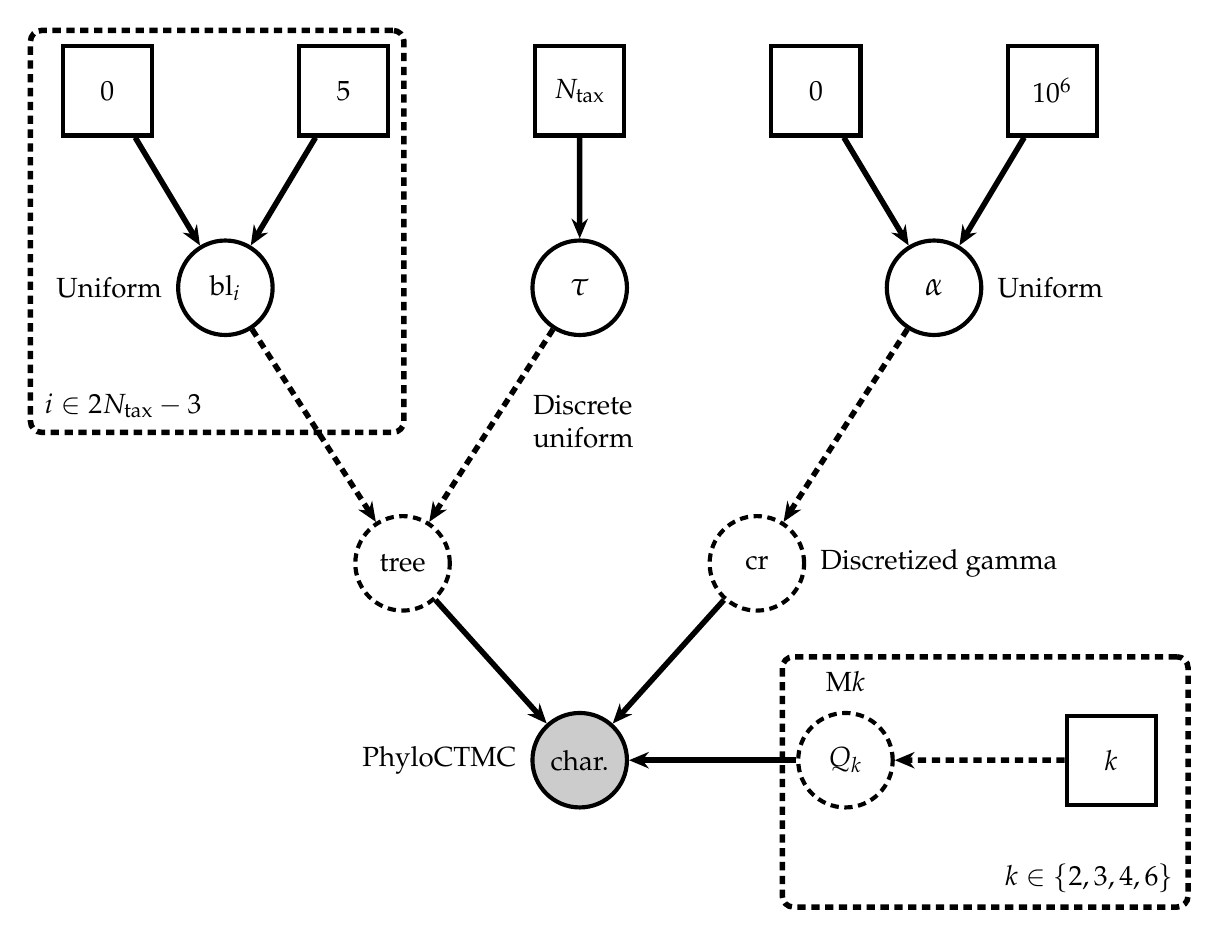
\begin{tikzpicture}
\node [constnode, minimum size=16mm] (unif00) at (0,2) {0};
\node [constnode, minimum size=16mm] (unif01) at (3,2) {5};
\node [constnode, minimum size=16mm] (unif10) at (9,2) {0};
\node [constnode, minimum size=16mm] (unif11) at (12,2) {$10^6$};
\node [constnode, minimum size=16mm] (N) at (6,2) {$N_{\text{tax}}$};
\node [stochnode, minimum size=12mm] (brlen) at (1.5,-0.5) {$\text{bl}_i$};
\node [stochnode, minimum size=12mm] (topology) at (6,-0.5) {\large $\tau$};
\node [stochnode, minimum size=12mm] (alpha) at (10.5,-0.5) {\large $\alpha$};
\node [detnode, minimum size=12mm] (tree) at (3.75,-4) {tree};
\node [detnode, minimum size=12mm] (gamma) at (8.25,-4) {cr};
\node [clampnode, minimum size=12mm] (char) at (6,-6.5) {char.};
\node [constnode, minimum size=16mm] (statenum) at (12.75,-6.5) {$k$};
\node [detnode, minimum size=12mm] (Q) at (9.375,-6.5) {$Q_k$};

\node [shape=rectangle, rounded corners=0mm, inner sep=0pt, anchor=west] (brlennumber) at (-0.8, -2) {$i \in 2N_{\text{tax}} - 3$};
\node [shape=rectangle, rounded corners=0mm, inner sep=0pt, anchor=east] (statenumber) at (13.55, -8) {$k \in \{2, 3, 4, 6\}$};
\node [shape=rectangle, rounded corners=0mm, inner sep=0pt, anchor=east] (distdescr0) at (0.7, -0.5) {Uniform};
\node [shape=rectangle, rounded corners=0mm, inner sep=0pt, anchor=west, align=left] (distdescr1) at (5.4, -2.2) {Discrete\\ uniform};
\node [shape=rectangle, rounded corners=0mm, inner sep=0pt, anchor=west] (distdescr2) at (11.3, -0.5) {Uniform};
\node [shape=rectangle, rounded corners=0mm, inner sep=0pt, anchor=west] (distdescr3) at (9.05, -4) {Discretized gamma};
\node [shape=rectangle, rounded corners=0mm, inner sep=0pt] (distdescr4) at (9.375, -5.5) {M$k$};
\node [shape=rectangle, rounded corners=0mm, inner sep=0pt, anchor=east] (distdescr5) at (5.2, -6.5) {PhyloCTMC};

\node [black, draw=black, line width=2pt, inner sep=5pt, shape=rectangle, rounded corners, densely dashed, fit = (distdescr0) (unif01) (brlennumber)] (brlenplate) {};
\node [black, draw=black, line width=2pt, inner sep=5pt, shape=rectangle, rounded corners, densely dashed, fit = (Q) (distdescr4) (statenumber)] (statenumplate) {};

\draw[-{Stealth[length=0.25cm, width=0.25cm, angle'=45]}, line width=2pt, color=black] (unif00) -- (brlen);
\draw[-{Stealth[length=0.25cm, width=0.25cm, angle'=45]}, line width=2pt, color=black] (unif01) -- (brlen);
\draw[-{Stealth[length=0.25cm, width=0.25cm, angle'=45]}, line width=2pt, color=black] (N) -- (topology);
\draw[-{Stealth[length=0.25cm, width=0.25cm, angle'=45]}, line width=2pt, color=black] (unif10) -- (alpha);
\draw[-{Stealth[length=0.25cm, width=0.25cm, angle'=45]}, line width=2pt, color=black] (unif11) -- (alpha);
\draw[-{Stealth[length=0.25cm, width=0.25cm, angle'=45]}, line width=2pt, densely dashed, color=black] (brlen) -- (tree);
\draw[-{Stealth[length=0.25cm, width=0.25cm, angle'=45]}, line width=2pt, densely dashed, color=black] (topology) -- (tree);
\draw[-{Stealth[length=0.25cm, width=0.25cm, angle'=45]}, line width=2pt, densely dashed, color=black] (alpha) -- (gamma);
\draw[-{Stealth[length=0.25cm, width=0.25cm, angle'=45]}, line width=2pt, densely dashed, color=black] (statenum) -- (Q);
\draw[-{Stealth[length=0.25cm, width=0.25cm, angle'=45]}, line width=2pt, color=black] (tree) -- (char);
\draw[-{Stealth[length=0.25cm, width=0.25cm, angle'=45]}, line width=2pt, color=black] (gamma) -- (char);
\draw[-{Stealth[length=0.25cm, width=0.25cm, angle'=45]}, line width=2pt, color=black] (Q) -- (char);
\end{tikzpicture}
}
\end{figure}

\noindent We see that the model itself has a tree-like shape: there are three separate branches that don't really communicate with each other, except that all of them ultimately enter the PhyloCTMC distribution from which we are drawing our character data. These are our submodels: let's highlight them and label them to make it clearer: \\[-0.75ex]

\begin{figure}[h]
\centering
\resizebox{!}{0.376\textheight}{
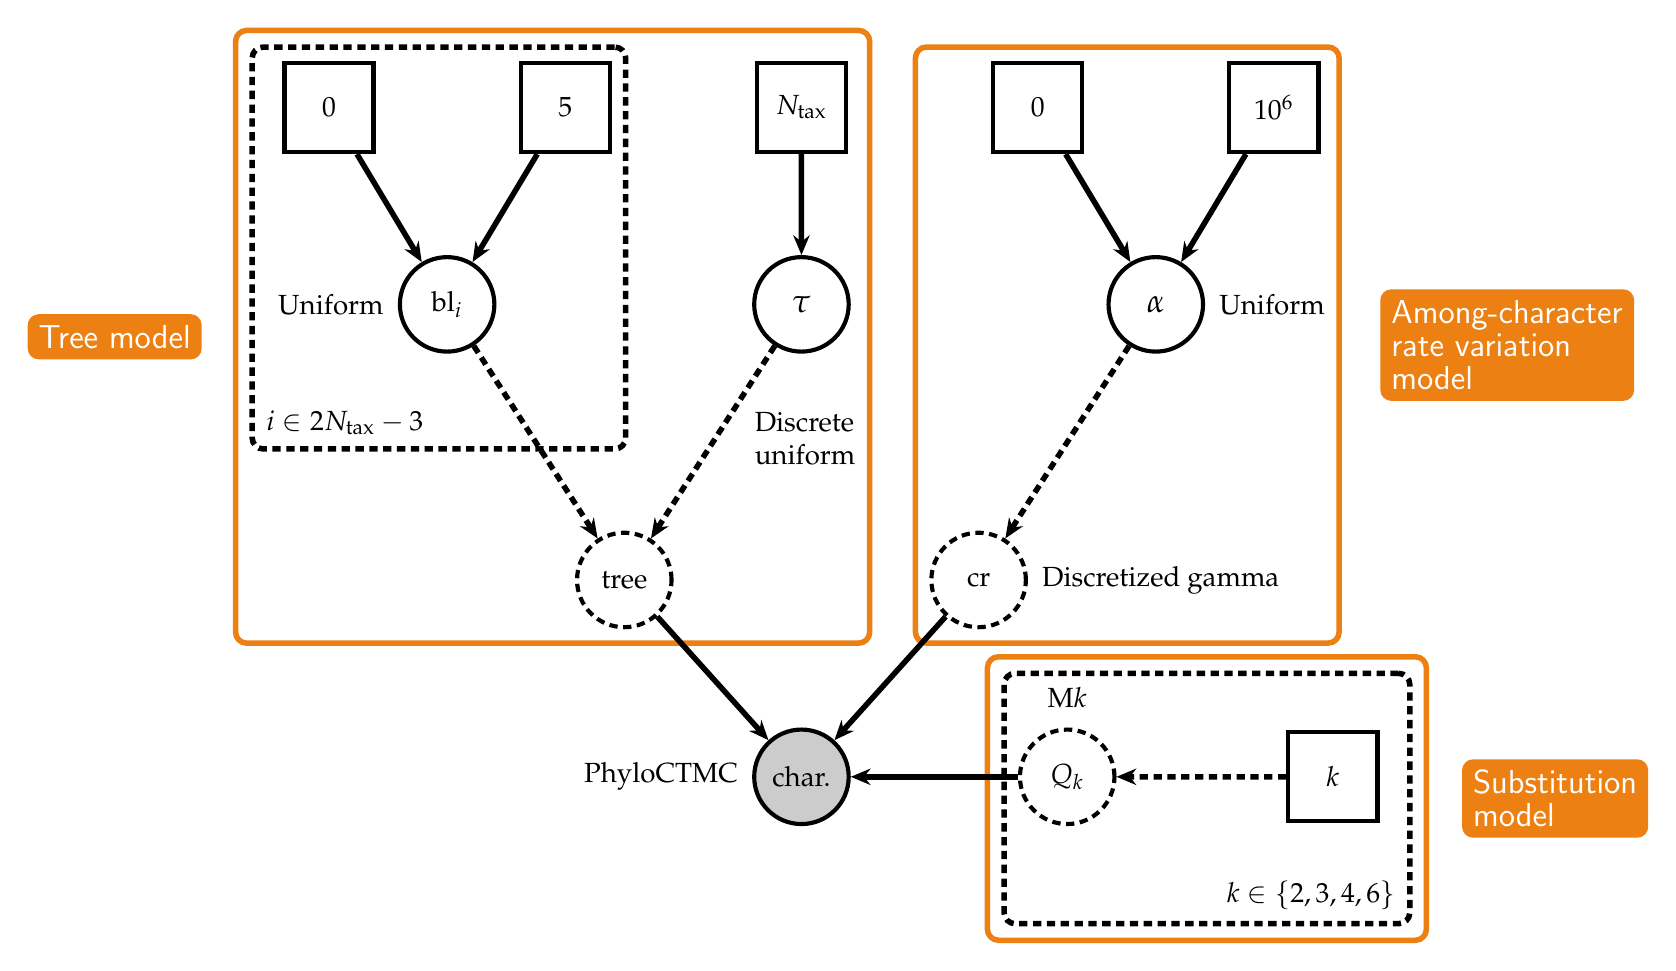
\begin{tikzpicture}
\node [constnode, minimum size=16mm] (unif00) at (0,2) {0};
\node [constnode, minimum size=16mm] (unif01) at (3,2) {5};
\node [constnode, minimum size=16mm] (unif10) at (9,2) {0};
\node [constnode, minimum size=16mm] (unif11) at (12,2) {$10^6$};
\node [constnode, minimum size=16mm] (N) at (6,2) {$N_{\text{tax}}$};
\node [stochnode, minimum size=12mm] (brlen) at (1.5,-0.5) {$\text{bl}_i$};
\node [stochnode, minimum size=12mm] (topology) at (6,-0.5) {\large $\tau$};
\node [stochnode, minimum size=12mm] (alpha) at (10.5,-0.5) {\large $\alpha$};
\node [detnode, minimum size=12mm] (tree) at (3.75,-4) {tree};
\node [detnode, minimum size=12mm] (gamma) at (8.25,-4) {cr};
\node [clampnode, minimum size=12mm] (char) at (6,-6.5) {char.};
\node [constnode, minimum size=16mm] (statenum) at (12.75,-6.5) {$k$};
\node [detnode, minimum size=12mm] (Q) at (9.375,-6.5) {$Q_k$};

\node [shape=rectangle, rounded corners=0mm, inner sep=0pt, anchor=west] (brlennumber) at (-0.8, -2) {$i \in 2N_{\text{tax}} - 3$};
\node [shape=rectangle, rounded corners=0mm, inner sep=0pt, anchor=east] (statenumber) at (13.55, -8) {$k \in \{2, 3, 4, 6\}$};
\node [shape=rectangle, rounded corners=0mm, inner sep=0pt, anchor=east] (distdescr0) at (0.7, -0.5) {Uniform};
\node [shape=rectangle, rounded corners=0mm, inner sep=0pt, anchor=west, align=left] (distdescr1) at (5.4, -2.2) {Discrete\\ uniform};
\node [shape=rectangle, rounded corners=0mm, inner sep=0pt, anchor=west] (distdescr2) at (11.3, -0.5) {Uniform};
\node [shape=rectangle, rounded corners=0mm, inner sep=0pt, anchor=west] (distdescr3) at (9.05, -4) {Discretized gamma};
\node [shape=rectangle, rounded corners=0mm, inner sep=0pt] (distdescr4) at (9.375, -5.5) {M$k$};
\node [shape=rectangle, rounded corners=0mm, inner sep=0pt, anchor=east] (distdescr5) at (5.2, -6.5) {PhyloCTMC};

\node [black, draw=black, line width=2pt, inner sep=5pt, shape=rectangle, rounded corners, densely dashed, fit = (distdescr0) (unif01) (brlennumber)] (brlenplate) {};
\node [black, draw=black, line width=2pt, inner sep=5pt, shape=rectangle, rounded corners, densely dashed, fit = (Q) (distdescr4) (statenumber)] (statenumplate) {};
\node [brown!30!orange, draw=brown!30!orange, line width=2pt, inner sep=5pt, shape=rectangle, rounded corners, fit = (brlenplate) (distdescr1) (tree)] (treemodel) {};
\node [brown!30!orange, draw=brown!30!orange, line width=2pt, inner sep=5pt, shape=rectangle, rounded corners, fit = (gamma) (distdescr2) (unif11)] (asrvmodel) {};
\node [brown!30!orange, draw=brown!30!orange, line width=2pt, inner sep=5pt, shape=rectangle, rounded corners, fit = (statenumplate)] (substmodel) {};
\node [shape=rectangle, rounded corners, inner sep=4pt, fill=brown!30!orange, text=white] (modeldescr0) at ($(treemodel.west)-(1.5,0)$) {\textsf{\large Tree model}};
\node [shape=rectangle, rounded corners, inner sep=4pt, fill=brown!30!orange, text=white, align=left] (modeldescr0) at ($(asrvmodel.east)-(-2.1,0)$) {\textsf{\large Among-character}\\ \textsf{\large rate variation}\\ \textsf{\large model}};
\node [shape=rectangle, rounded corners, inner sep=4pt, fill=brown!30!orange, text=white, align=left] (modeldescr0) at ($(substmodel.east)-(-1.6,0)$) {\textsf{\large Substitution}\\ \textsf{\large model}};

\draw[-{Stealth[length=0.25cm, width=0.25cm, angle'=45]}, line width=2pt, color=black] (unif00) -- (brlen);
\draw[-{Stealth[length=0.25cm, width=0.25cm, angle'=45]}, line width=2pt, color=black] (unif01) -- (brlen);
\draw[-{Stealth[length=0.25cm, width=0.25cm, angle'=45]}, line width=2pt, color=black] (N) -- (topology);
\draw[-{Stealth[length=0.25cm, width=0.25cm, angle'=45]}, line width=2pt, color=black] (unif10) -- (alpha);
\draw[-{Stealth[length=0.25cm, width=0.25cm, angle'=45]}, line width=2pt, color=black] (unif11) -- (alpha);
\draw[-{Stealth[length=0.25cm, width=0.25cm, angle'=45]}, line width=2pt, densely dashed, color=black] (brlen) -- (tree);
\draw[-{Stealth[length=0.25cm, width=0.25cm, angle'=45]}, line width=2pt, densely dashed, color=black] (topology) -- (tree);
\draw[-{Stealth[length=0.25cm, width=0.25cm, angle'=45]}, line width=2pt, densely dashed, color=black] (alpha) -- (gamma);
\draw[-{Stealth[length=0.25cm, width=0.25cm, angle'=45]}, line width=2pt, densely dashed, color=black] (statenum) -- (Q);
\draw[-{Stealth[length=0.25cm, width=0.25cm, angle'=45]}, line width=2pt, color=black] (tree) -- (char);
\draw[-{Stealth[length=0.25cm, width=0.25cm, angle'=45]}, line width=2pt, color=black] (gamma) -- (char);
\draw[-{Stealth[length=0.25cm, width=0.25cm, angle'=45]}, line width=2pt, color=black] (Q) -- (char);
\end{tikzpicture}
}
\end{figure}

\newpage

\noindent You may have also noticed this modular nature of our model in the corresponding Rev script (\texttt{Tedford\_phylo.Rev}), which used subheadings for the individual submodels: \\[2ex]

\indent \texttt{\#\#\#\#\#\#\#\#\#\#\#\#\#\#\#\#\#\#\#\#\#\#\#\#\#\#\#\#\#\#} \\
\indent \texttt{\# Topology and branch lengths \#} \\
\indent \texttt{\#\#\#\#\#\#\#\#\#\#\#\#\#\#\#\#\#\#\#\#\#\#\#\#\#\#\#\#\#\#} \\
\ \\
\indent \texttt{\vdots} \\
\ \\
\indent \texttt{\#\#\#\#\#\#\#\#\#\#\#\#\#\#\#\#\#\#\#\#\#\#\#\#\#\#\#\#\#\#\#\#\#\#\#} \\
\indent \texttt{\# Rate variation across characters \#} \\
\indent \texttt{\#\#\#\#\#\#\#\#\#\#\#\#\#\#\#\#\#\#\#\#\#\#\#\#\#\#\#\#\#\#\#\#\#\#\#} \\
\ \\
\indent \texttt{\vdots} \\
\ \\
\indent \texttt{\#\#\#\#\#\#\#\#\#\#\#\#\#\#\#\#\#\#\#\#\#\#\#\#\#\#\#\#\#\#\#\#\#\#\#\#\#\#\#\#\#\#\#\#\#\#\#\#\#\#\#\#\#\#\#\#\#} \\
\indent \texttt{\# Mk substitution models, partitioned by number of states \#} \\
\indent \texttt{\#\#\#\#\#\#\#\#\#\#\#\#\#\#\#\#\#\#\#\#\#\#\#\#\#\#\#\#\#\#\#\#\#\#\#\#\#\#\#\#\#\#\#\#\#\#\#\#\#\#\#\#\#\#\#\#\#} \\[2ex]

\noindent The whole trick behind switching from inferring phylograms to inferring chronograms consists in (1) replacing the tree submodel and (2) adding a new submodel corresponding to our relaxed clock. We can keep everything else as-is, including the substitution and among-character rate variation models, as well as the MCMC machinery under the hood.

\section*{The Fossilized Birth-Death model}

\vspace*{0.5ex}

\begin{center}
\textcolor{blue}{What follows has been adapted from a BEAST 2 tutorial developed by Prof. Tracy Heath's lab at the Iowa State University. You can access the full version from \\
\url{https://taming-the-beast.org/tutorials/FBD-tutorial/FBD-tutorial.pdf}. \\
BEAST 2 is a program similar to RevBayes, but unlike the latter, it can only infer chronograms, not phylograms.}
\end{center}

\vspace*{1ex}

\noindent The new tree model we are going to be using is called the Fossilized Birth-Death (FBD) model. It was described by Tracy Heath and colleagues in 2014, building upon earlier work by Tanja Stadler. As its name suggests, the FBD model considers a phylogenetic tree to be the product of three processes: the ``birth'' of new lineages, or speciation; the ``death'' of lineages, or extinction; and the fossilization process, by which we come to learn about lineages that did not survive to the present. It further assumes that the waiting times between the successive occurrences of the same kind of event (e.g., between two speciations, two extinctions, etc.) are exponentially distributed, making short waiting times more likely than long waiting times. In total, the model has five parameters: \\

\begin{table}[h]
\centering
\begin{tabular}{ll}
\toprule
\textbf{Parameter} & \textbf{Description} \\
\midrule
$\lambda$ & Speciation rate \\
$\mu$ & Extinction rate \\
$\psi$ & Fossil recovery rate \\
$\rho$ & Probability of sampling extant species \\
$t_o$ & Time of origin \\
\bottomrule
\end{tabular}
\label{table1}
\end{table}

\vspace*{-3ex}

\noindent Instead of dealing with the three rates $\lambda$, $\mu$, $\psi$ directly, however, it is often more convenient to \textit{reparameterize} the FBD model. The concept of reparameterization is analogous to the idea of different coordinate systems. When it comes to locating a point on a two-dimensional plane, most of us would probably use two orthogonal axes, $x$ and $y$. However, we could also employ, say, the polar coordinate system, which relies on radial distance $r$ from a reference point and angle $\phi$ relative to a reference direction. Both descriptions are valid, both have the same expressive power, and both are equally complex in that they require two coordinates: ($x$, $y$) or ($r$, $\phi$). The same is true of reparameterization. The reason why we do this with the FBD model is that two of the three new parameters range from 0 to 1, which makes it easier to place uninformative priors on them:

% Credit: Will Robertson, https://tex.stackexchange.com/a/4024
\renewcommand{\thetable}{2}
\refstepcounter{table}
\begin{table}[h]
\centering
\begin{tabular}{ll}
\toprule
\textbf{Reparameterization} & \textbf{Description} \\
\midrule
$d = \lambda - \mu$ & Net diversification rate \\
$r = \frac{\mu}{\lambda}$ & Extinction fraction \\
$s = \frac{\psi}{\mu + \psi}$ & Probability a species leaves behind a fossil before going extinct \\
\bottomrule
\end{tabular}
\label{table2}
\end{table}

\noindent The remaining two parameters stay the same, yielding the following model:

\begin{figure}[h]
\centering
\resizebox{!}{0.39\textheight}{
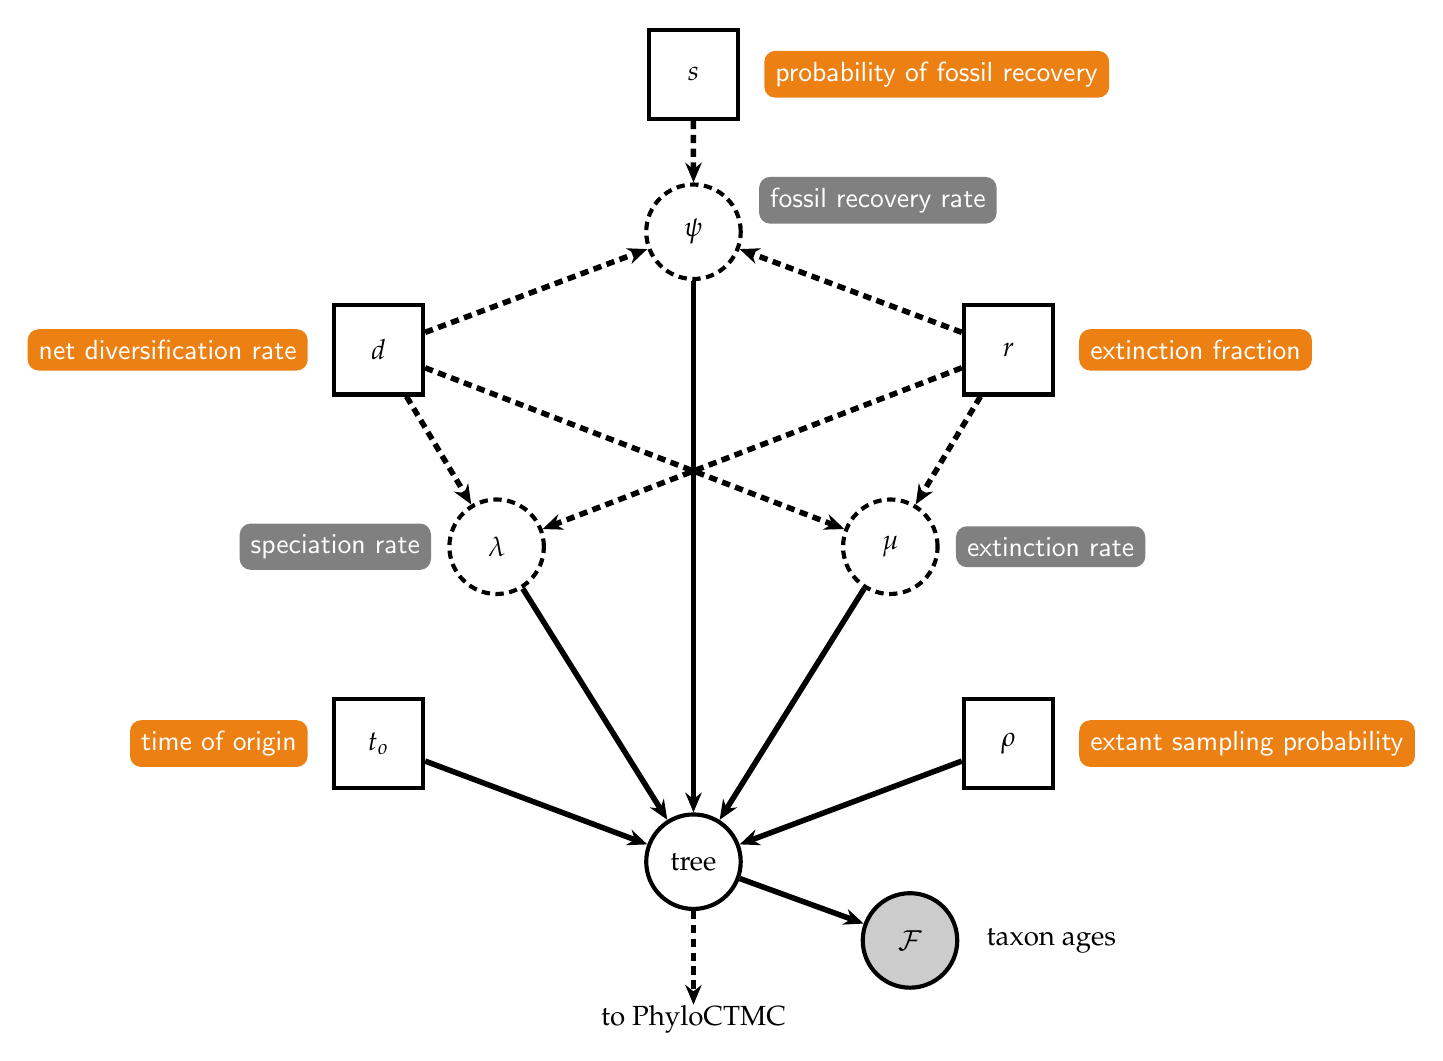
\begin{tikzpicture}
\node [constnode, minimum size=16mm] (s) at (0,2) {$s$};
\node [detnode, minimum size=12mm] (psi) at (0,0) {$\psi$};
\node [constnode, minimum size=16mm] (d) at (-4,-1.5) {$d$};
\node [constnode, minimum size=16mm] (r) at (4,-1.5) {$r$};
\node [stochnode, minimum size=12mm] (tree) at (0,-8) {tree};
\node [detnode, minimum size=12mm] (lambda) at (-2.5,-4) {$\lambda$};
\node [detnode, minimum size=12mm] (mu) at (2.5,-4) {$\mu$};
\node [constnode, minimum size=16mm] (to) at (-4,-6.5) {$t_o$};
\node [constnode, minimum size=16mm] (rho) at (4,-6.5) {$\rho$};
\node [clampnode, minimum size=12mm] (occ) at (2.75,-9) {$\mathcal{F}$};
\node [shape=rectangle, rounded corners=0mm, inner sep=0pt, align=center] (out) at (0, -10) {to PhyloCTMC};

\draw[-{Stealth[length=0.25cm, width=0.25cm, angle'=45]}, line width=2pt, color=black] (psi) -- (tree);
\draw[-{Stealth[length=0.25cm, width=0.25cm, angle'=45]}, line width=2pt, color=black] (lambda) -- (tree);
\draw[-{Stealth[length=0.25cm, width=0.25cm, angle'=45]}, line width=2pt, color=black] (mu) -- (tree);
\draw[-{Stealth[length=0.25cm, width=0.25cm, angle'=45]}, line width=2pt, color=black] (to) -- (tree);
\draw[-{Stealth[length=0.25cm, width=0.25cm, angle'=45]}, line width=2pt, color=black] (rho) -- (tree);
\draw[-{Stealth[length=0.25cm, width=0.25cm, angle'=45]}, line width=2pt, color=black] (tree) -- (occ);
\draw[-{Stealth[length=0.25cm, width=0.25cm, angle'=45]}, line width=2pt, densely dashed, color=black] (s) -- (psi);
\draw[-{Stealth[length=0.25cm, width=0.25cm, angle'=45]}, line width=2pt, densely dashed, color=black] (d) -- (psi);
\draw[-{Stealth[length=0.25cm, width=0.25cm, angle'=45]}, line width=2pt, densely dashed, color=black] (r) -- (psi);
\draw[-{Stealth[length=0.25cm, width=0.25cm, angle'=45]}, line width=2pt, densely dashed, color=black] (d) -- (lambda);
\draw[-{Stealth[length=0.25cm, width=0.25cm, angle'=45]}, line width=2pt, densely dashed, color=black] (d) -- (mu);
\draw[-{Stealth[length=0.25cm, width=0.25cm, angle'=45]}, line width=2pt, densely dashed, color=black] (r) -- (lambda);
\draw[-{Stealth[length=0.25cm, width=0.25cm, angle'=45]}, line width=2pt, densely dashed, color=black] (r) -- (mu);
\draw[-{Stealth[length=0.25cm, width=0.25cm, angle'=45]}, line width=2pt, densely dashed, color=black] (tree) -- (out);

\node [shape=rectangle, rounded corners, inner sep=4pt, fill=brown!30!orange, text=white, align=left, anchor=west] (descr0) at ($(s.east)-(-0.3,0)$) {\textsf{probability of fossil recovery}};
\node [shape=rectangle, rounded corners, inner sep=4pt, fill=brown!30!orange, text=white, align=left, anchor=east] (descr1) at ($(d.west)-(0.3,0)$) {\textsf{net diversification rate}};
\node [shape=rectangle, rounded corners, inner sep=4pt, fill=brown!30!orange, text=white, align=left, anchor=west] (descr2) at ($(r.east)-(-0.3,0)$) {\textsf{extinction fraction}};
\node [shape=rectangle, rounded corners, inner sep=4pt, fill=brown!30!orange, text=white, align=left, anchor=east] (descr3) at ($(to.west)-(0.3,0)$) {\textsf{time of origin}};
\node [shape=rectangle, rounded corners, inner sep=4pt, fill=brown!30!orange, text=white, align=left, anchor=west] (descr4) at ($(rho.east)-(-0.3,0)$) {\textsf{extant sampling probability}};
\node [shape=rectangle, rounded corners, inner sep=4pt, fill=gray, text=white, align=left, anchor=west] (descr5) at ($(psi.east)-(-0.2,-0.4)$) {\textsf{fossil recovery rate}};
\node [shape=rectangle, rounded corners, inner sep=4pt, fill=gray, text=white, align=left, anchor=east] (descr6) at ($(lambda.west)-(0.2,0)$) {\textsf{speciation rate}};
\node [shape=rectangle, rounded corners, inner sep=4pt, fill=gray, text=white, align=left, anchor=west] (descr7) at ($(mu.east)-(-0.2,0)$) {\textsf{extinction rate}};
\node [shape=rectangle, rounded corners=0mm, inner sep=4pt, anchor=west] (out) at ($(occ.east)-(-0.2,0)$) {taxon ages};
\end{tikzpicture}
}
\end{figure}

\noindent And that's before we even placed priors on the free parameters -- you can tell that things are starting to get a bit complicated! \\

\noindent Before we begin translating this model into Rev, we should notice that a new clamped variable appeared in the graph. Previously, only the characters (drawn from PhyloCTMC) were clamped. That makes sense in light of what we said above: estimating chronograms requires additional data in the form of taxon ages. However, this raises a question of how we can load such data into RevBayes. It turns out there are two things RevBayes absolutely insists on:

\begin{enumerate}
  \setlength\itemsep{-0.3em}
  \item Your data must consist of three columns, called (in this order): \texttt{taxon}, \texttt{min\_age}, and \texttt{max\_age};
  \item The entries in your \texttt{taxon} column must perfectly match the taxon names in your Nexus file.
\end{enumerate}

\noindent I like to keep my age data in a tab-separated file. When I open the file I assembled for the Tedford et al. dataset in a text editor (e.g., TextEdit on macOS, Notepad on Windows, Gedit on Linux), its first few lines look as follows: \\

\indent \texttt{taxon\ \ \ \ min\_age max\_age} \\
\indent \texttt{Hesperocyoninae 15.0\ \ \ \ 40.0} \\
\indent \texttt{Borophaginae	\ \ \ \ 2.0\ \ \ \ \	34.0} \\
\indent \texttt{Leptocyon\_mollis\ \ \ \ \ \ \ \ \ 29.0\ \ \ \ 30.0} \\
\indent \texttt{Leptocyon\_douglassi\ \ \ \ \,\ 25.7\ \ \ \ 30.6} \\

\begin{center}
\textcolor{red}{For your convenience, I uploaded an example file with the Tedford et al. age data to Canvas (\texttt{Tedford\_ages.tsv}).}
\end{center}

\noindent This is how to load a file like this into RevBayes: \\

\indent \texttt{taxa <- readTaxonData("/Users/David/Tedford\_ages.tsv")} \\

\noindent Next, let's place priors on the three rate parameters of the FBD model. The extinction fraction and the fossil recovery probability range from 0 to 1, so in the absence of any meaningful prior information, the uniform distribution $U(0,1)$ is the natural choice. The net diversification rate, on the other hand, ranges from 0 to infinity. We'll just use an exponential prior distribution with a rate of 10, corresponding to a mean of 1/10 = 0.1 species per million years. (Remember, this is the rate of species build-up, i.e., excess of speciation over extinction.) \\

\indent \texttt{diversification {\footnotesize $\sim$} dnExponential(10)} \\
\indent \texttt{ext\_frac {\footnotesize $\sim$} dnUniform(0, 1)} \\
\indent \texttt{fossil\_prob {\footnotesize $\sim$} dnUniform(0, 1)} \\

\noindent One trick that can improve parameter space exploration for very complex models is to use multiple moves of the same kind, but with different tuning values. That way, some will be bolder and favor long leaps, while others will be more conservative and keep close to the current value: \\

\indent \texttt{\# Specify a scale move on the diversification parameter} \\
\indent \texttt{moves.append( mvScale(diversification, lambda=0.01, weight=5) )} \\
\indent \texttt{moves.append( mvScale(diversification, lambda=0.1,\ \,\ weight=3) )} \\
\indent \texttt{moves.append( mvScale(diversification, lambda=1,\ \ \ \,\,\ weight=1) )} \\
\ \\
\indent \texttt{\# Specify a sliding-window move on the ext\_frac parameter} \\
\indent \texttt{moves.append( mvSlide(ext\_frac, delta=0.01, weight=5) )} \\
\indent \texttt{moves.append( mvSlide(ext\_frac, delta=0.1,\ \,\ weight=3) )} \\
\indent \texttt{moves.append( mvSlide(ext\_frac, delta=1,\ \ \ \,\,\ weight=1) )} \\
\ \\
\indent \texttt{\# Specify a sliding-window move on the fossil\_prob parameter} \\
\indent \texttt{moves.append( mvSlide(fossil\_prob, delta=0.01, weight=5) )} \\
\indent \texttt{moves.append( mvSlide(fossil\_prob, delta=0.1,\ \,\ weight=3) )} \\
\indent \texttt{moves.append( mvSlide(fossil\_prob, delta=1,\ \ \ \,\,\ weight=1) )} \\ 

\noindent Next, reparameterize. If it's not clear to you what's happening below, go back to Table~\ref{table2} and think about how you could recover $\lambda$, $\mu$, $\psi$ from $d$, $r$, $s$: \\

\indent \texttt{speciation := diversification / abs(1.0 - ext\_frac)} \\ 
\indent \texttt{extinction := (ext\_frac * diversification) / abs(1.0 - ext\_frac)} \\ 
\indent \texttt{recovery := (fossil\_prob / abs(1.0 - fossil\_prob)) * extinction} \\ 

\noindent An interesting feature of the FBD model is that it is not identifiable when all of its parameters are left free, just like rate and time were not identifiable when we were trying to estimate them from character data alone. To avoid this problem, we can pick one parameter and set it to a fixed value. Fortunately, there is a natural choice for the parameter to be fixed: it would be the extant sampling probability $\rho$. As long as we have a good idea of how many extant species there are in our group of interest, we can treat this parameter as being known without error. For example, Wikipedia says there are 34 extant species of canids. The Tedford et al. (2009) matrix includes 7 of them, so we can do the following: \\

\indent \texttt{rho <- 7/34} \\

\noindent The only remaining parameter we have to place a prior on is the time of origin of our time tree. Here, it actually bears reflecting on our prior beliefs in a little more detail. We know that the origin of a clade is likely to somewhat predate its first appearance in the fossil record. We can then think of the problem in terms of the expected waiting time between these two events (i.e., origin vs. first appearance). If the fossil record of our group is very good, the expected waiting time will be quite short. If, on the other hand, our fossil record is sparse, the waiting time could be pretty long. The canid fossil record is very good in comparison to most other vertebrates, so we would expect the former. But how short exactly? Fortunately, this happens to be one of the cases where we do, in fact, have some prior information we can use. According to a \href{https://royalsocietypublishing.org/doi/epdf/10.1098/rspb.2012.0683}{2012 study by Mario dos Reis and colleagues}, the family Canidae diverged from its sister group approximately 49 million years ago. The earliest canid fossil, \textit{Hesperocyon}, is about 38 million years old. We might therefore want to place, say, 95\% probability on origin times that lie between these two values, followed by a long, low-probability tail for ages older than 49 million years. \\

\noindent A good choice would be an \textit{offset exponential} distribution, which looks and behaves just like a regular exponential distribution, except that its support is $[L, \infty)$ rather than $[0, \infty)$, with $L$ being some arbitrary positive number. Here, we set it to 38, because the canid clade cannot be younger than its oldest known fossil. All that's left to do is determine what the mean of our exponential has to be in order for its 95th percentile to equal 49. We can do this using the quantile function \texttt{qexp()}, which finds a time $T$ such that the probability $P(t_o \leq T)$ equals a specified value (here, 0.95): \\

\indent \texttt{mean\_prior\_age <- (49 - 38)/qexp(0.95)} \\
\indent \texttt{\# The lambda parameter of an exponential function is the inverse of the mean:} \\
\indent \texttt{origin\_time {\footnotesize $\sim$} dnExponential(lambda=1/mean\_prior\_age, offset=38)} \\

\noindent This is what our prior looks like:

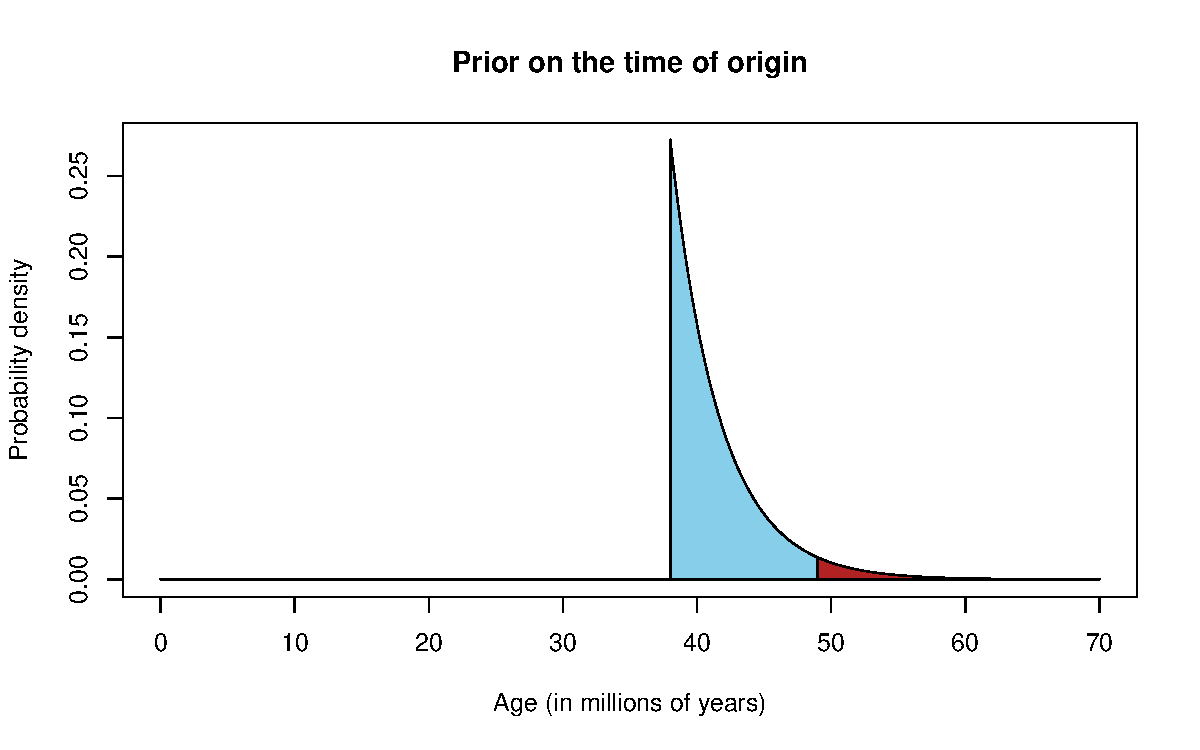
\includegraphics[width=\textwidth]{timeoforiginprior.pdf}

\noindent Note that 95\% of the total probability mass is contained in the region highlighted in blue, while the red tail extends all the way to positive infinity. \\

\noindent Let's not forget that the time of origin, too, is a parameter we want to estimate, so we have to place a move on it: \\

\indent \texttt{\# Specify a sliding-window move on the origin\_time parameter} \\
\indent \texttt{moves.append( mvSlide(origin\_time, delta=1, weight=10) )} \\

\noindent Now we just put everything together using the \texttt{dnFBDP()} function. (You could also use its longer but more descriptive alias, \texttt{dnFossilizedBirthDeath()}.) \\

\indent \texttt{tree {\footnotesize $\sim$} dnFBDP(origin=origin\_time, lambda=speciation, mu=extinction,} \\
\indent \texttt{\ \ \ \,\ \ \ \ \ \ \ \ \ \ \ \ \ \ psi=recovery, rho=rho, taxa=taxa)} \\

\noindent We have to use a different set of moves now that we are inferring a time tree (chronogram) rather than a branch-length tree (phylogram): \\

\indent \texttt{\# Specify moves on topology; allow some taxa to be ancestors of others} \\
\indent \texttt{moves.append( mvFNPR(tree, weight=15) )} \\
\indent \texttt{moves.append( mvCollapseExpandFossilBranch(tree, origin\_time, weight=6) )} \\
\ \\
\indent \texttt{\# Specify moves on the node ages, including the root age} \\
\indent \texttt{moves.append( mvNodeTimeSlideUniform(tree, weight=40) )} \\
\indent \texttt{moves.append( mvRootTimeSlideUniform(tree, origin\_time, weight=5) )} \\

\noindent This highlights another cool feature of the FBD model. So far, we have restricted ourselves to inferring sister-group relationships, but we had nothing to say about ancestor-descendant relationships. In a PAUP* cladogram or even a RevBayes phylogram, you'll never see one taxon being directly ancestral to another, even if that was in fact their true relationship. The best we could have done in such a situation was to place the ancestor in a sister-group relationship with the clade formed by its descendants, and make its branch very, very short to indicate that it did not undergo any changes aside from those that were also shared by its descendants. With FBD time trees, however, there are no such limitations, and we can infer ancestor-descendant relationships to our heart's content. Let's ask RevBayes how many ancestors it found among the 39 canid taxa in our sample: \\

\indent \texttt{num\_samp\_anc := tree.numSampledAncestors()}

\section*{Strict clock}

Compared to the FBD model, setting up a strict clock in RevBayes is a breeze. We just need to specify a prior on our \textit{clock rate}, that is, the ``base'' rate of character change, which gets further scaled up and down by our among-character rate variation model. We will use a \href{https://en.wikipedia.org/wiki/Log-normal_distribution}{lognormal distribution} for this purpose. This is the distribution followed by a stochastic variable whose logarithm is normally distributed. The lognormal distribution has support on $[0, \infty)$ and is fully specified by two parameters, namely the log-scale mean $\mu$ and the log-scale standard deviation $\sigma$. We back-derive the log-scale mean from the actual mean, which we simply set equal to a value that seems reasonable to us: 0.005 changes per character per million years. Our choice of $\sigma$ probably seems completely arbitrary, but there is a reason behind it: this way, 95\% prior probability is going to span exactly two orders of magnitude. \\

\indent \texttt{sigma <- 1.17481} \\
\indent \texttt{clock\_mean <- 0.005} \\
\indent \texttt{mu := ln(clock\_mean) - (0.5 * sigma\textasciicircum 2)} \\
\indent \texttt{clock\_rate {\footnotesize $\sim$} dnLognormal(mean=mu, sd=sigma)} \\
\ \\
\indent \texttt{\# Specify a scale move on the clock rate parameter} \\
\indent \texttt{moves.append( mvScale(clock\_rate, lambda=1, weight=10) )} \\

\noindent This is what our strict clock model looks like: \\

\begin{figure}[h]
\centering
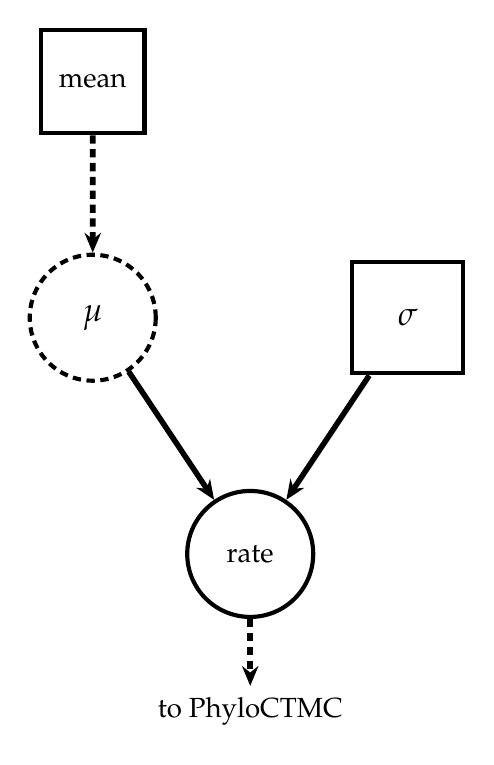
\begin{tikzpicture}
\node [constnode, minimum size=16mm] (mean) at (0,2) {mean};
\node [constnode, minimum size=20mm] (sigma) at (4,-1) {\large $\sigma$};
\node [detnode, minimum size=16mm] (mu) at (0,-1) {\large $\mu$};
\node [stochnode, minimum size=16mm] (rate) at (2,-4) {rate};
\node [shape=rectangle, rounded corners=0mm, inner sep=4pt, align=center] (out) at (2, -6) {to PhyloCTMC};

\draw[-{Stealth[length=0.25cm, width=0.25cm, angle'=45]}, line width=2pt, color=black] (mu) -- (rate);
\draw[-{Stealth[length=0.25cm, width=0.25cm, angle'=45]}, line width=2pt, color=black] (sigma) -- (rate);
\draw[-{Stealth[length=0.25cm, width=0.25cm, angle'=45]}, line width=2pt, densely dashed, color=black] (mean) -- (mu);
\draw[-{Stealth[length=0.25cm, width=0.25cm, angle'=45]}, line width=2pt, densely dashed, color=black] (rate) -- (out);
\end{tikzpicture}
\end{figure}

\noindent Our specification of PhyloCTMC also has to change to account for the fact that we are now adding branch rates as a new submodel of our overall model: \\

\indent \texttt{characters[j] {\footnotesize $\sim$} dnPhyloCTMC(tree=tree, Q=Q[j], type="Standard",} \\
\indent \texttt{\ \ \ \ \ \ \ \ \ \ \ \ \ \ \ \ \ \ \ \ \ \ \ \ \ \ \ \ \ \ \ \ \ \ \ branchRates=clock\_rate, siteRates=char\_rates,} \\
\indent \texttt{\ \ \ \ \ \ \ \ \ \ \ \ \ \ \ \ \ \ \ \ \ \ \ \ \ \ \ \ \ \ \ \ \ \ \ coding="variable")} \\

\noindent RevBayes is smart enough to automatically apply the \texttt{clock\_rate} value to every single branch in our tree. Interestingly, here we encounter another subtle difference between cladograms or phylograms on the one hand, and chronograms on the other. Our cladograms and phylograms were \textit{unrooted}, and as a result, had $2N - 3$ branches for every $N$ taxa. However, the FBD model (or indeed, any other tree model that allows us to infer time trees) induces a prior probability distribution on \textit{rooted} trees, which have an extra root branch, and thus $2N - 2$ branches in total.

\begin{center}
\textcolor{red}{For your convenience, all of the above code has been packaged into a single Rev script available from Canvas (\texttt{Tedford\_FBD\_strictclock.Rev}).}
\end{center}

\vspace*{1ex}

\hrule
\ \\[1ex]
\textbf{1) Run a strict-clock time tree analysis on your pasta dataset. If you want, you can use the \texttt{Tedford\_FBD\_strictclock.Rev} script as a template. Think about which parts of the code are generally applicable, and which you’ll need to tailor to your own data. You might want to increase the number of MCMC generations compared to the 20,000 we used in Lab 7. Why do you think that is?} \\

\noindent \textbf{2) Did your parameters reach stationarity? Which, if any, don't look good?} \\

\noindent \textbf{3) We specified priors on the clock rate, net diversification rate, extinction fraction, and extant sampling probability. What do their posteriors look like? (Tip: in Tracer, click on the ``Estimates'' tab to get their mean and 95\% credibility interval.) How do the posteriors compare to the priors we used?} \\

\noindent \textbf{4) Generate the MCC and/or MAP summary tree for your analysis, visualize it, and include the resulting image in your answer sheet. How does it compare to your trees from the previous weeks? Briefly describe its topology, divergence times, and posterior probabilities.} \\

\noindent \textbf{5) Does your summary tree contain any ancestor-descendant relationships? If so, what are they? What is the posterior mean for the number of sampled ancestors in your tree?} \\
\hrule

\section*{Uncorrelated lognormal relaxed clock}

Trying our hand at time tree estimation using the strict clock was fun, but as we've learned above, relaxed clock models is where it's really at. Let's set up an \textit{uncorrelated lognormal} (UCLN) model, which is one of the most commonly used relaxed clocks. The word ``lognormal'' indicates that the rates of character change for each branch will be drawn from a lognormal distribution. The word ``uncorrelated'' means that each branch draws its rate independently from the same distribution. There are also \textit{autocorrelated} models, which assume that the rate of any given branch tends to stay close to the rate of its parent branch, and that it takes time for large rate differences to evolve along the tree. In uncorrelated models, this isn't necessarily true: very slow and very fast branches can directly adjoin each other, because they all draw their rates independently. There is an ongoing debate about the relative merits of uncorrelated and autocorrelated clock models.

\noindent We already know how to parameterize a lognormal distribution, so we just need to come up with appropriate priors on $\mu$ and $\sigma$: \\

\indent \texttt{\# The exponential prior below ensures that the mean of the prior on the} \\
\indent \texttt{\# mean clock rate will be equal to 0.03, six times greater than before.} \\
\indent \texttt{ucln\_mean {\footnotesize $\sim$} dnExponential(33.3)} \\
\ \\
\indent \texttt{\# The log-scale standard deviation of our branch rate distribution will} \\
\indent \texttt{\# also be exponentially distributed:} \\
\indent \texttt{ucln\_sigma {\footnotesize $\sim$} dnExponential(1.0)} \\
\ \\
\indent \texttt{ucln\_mu := ln(ucln\_mean) - (0.5 * ucln\_sigma\textasciicircum 2)} \\
\indent \texttt{moves.append( mvScale(ucln\_mean, lambda=1.0, weight=4))} \\
\indent \texttt{moves.append( mvScale(ucln\_sigma, lambda=0.5, weight=4))} \\

\noindent We also know that each branch rate is going to represent an independent draw from the distribution we have just defined. A \texttt{for} loop is an appropriate construct for this: \\

\indent \texttt{for (i in 1:num\_branches) \{} \\
\indent \texttt{\ \ \ \ branch\_rates[i] {\footnotesize $\sim$} dnLognormal(ucln\_mu, ucln\_sigma)} \\
\indent \texttt{\ \ \ \ moves.append( mvScale(branch\_rates[i], lambda=1, weight=2) )} \\
\indent \texttt{\}} \\

\noindent This is what our UCLN model looks like: \\

\begin{figure}[h]
\centering
\resizebox{!}{0.42\textheight}{
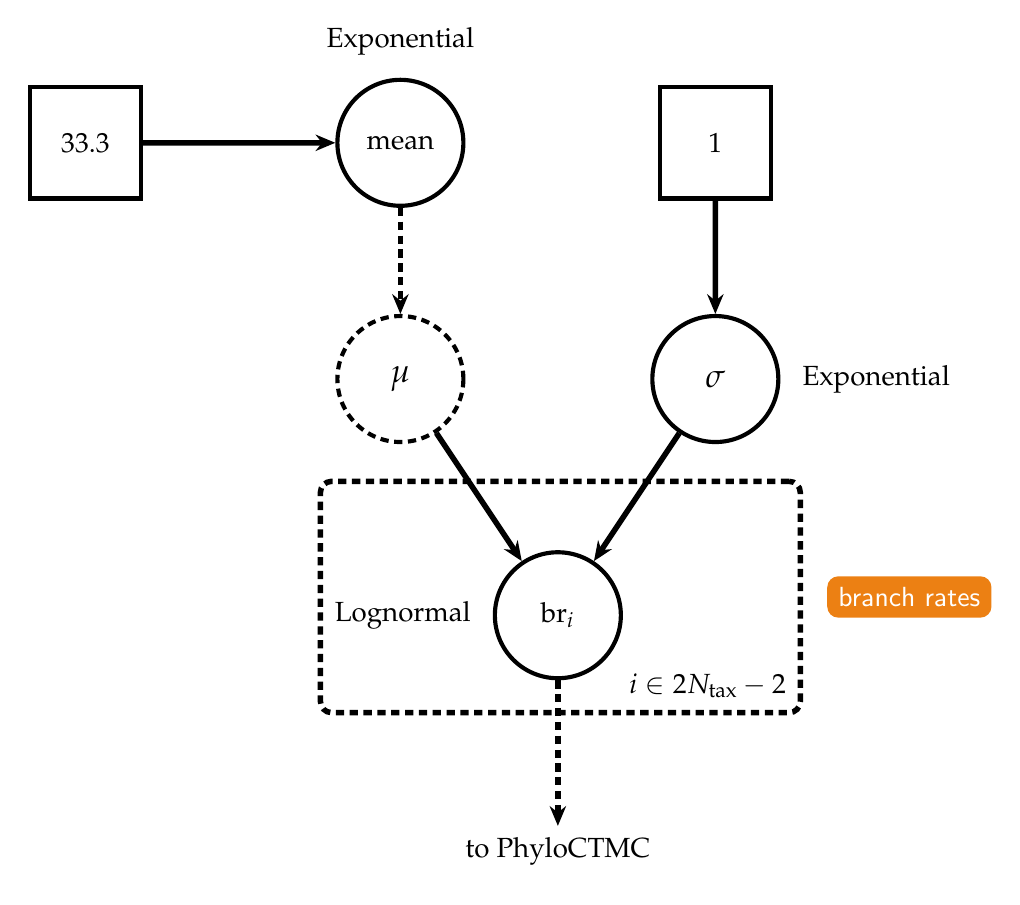
\begin{tikzpicture}
\node [constnode, minimum size=20mm] (exp0) at (-4,2) {33.3};
\node [constnode, minimum size=20mm] (exp1) at (4,2) {1};
\node [stochnode, minimum size=16mm] (mean) at (0,2) {mean};
\node [stochnode, minimum size=16mm] (sigma) at (4,-1) {\large $\sigma$};
\node [detnode, minimum size=16mm] (mu) at (0,-1) {\large $\mu$};
\node [stochnode, minimum size=16mm] (rate) at (2,-4) {$\text{br}_i$};
\node [shape=rectangle, rounded corners=0mm, inner sep=4pt, align=center] (out) at (2, -7) {to PhyloCTMC};

\draw[-{Stealth[length=0.25cm, width=0.25cm, angle'=45]}, line width=2pt, color=black] (exp0) -- (mean);
\draw[-{Stealth[length=0.25cm, width=0.25cm, angle'=45]}, line width=2pt, color=black] (exp1) -- (sigma);
\draw[-{Stealth[length=0.25cm, width=0.25cm, angle'=45]}, line width=2pt, color=black] (mu) -- (rate);
\draw[-{Stealth[length=0.25cm, width=0.25cm, angle'=45]}, line width=2pt, color=black] (sigma) -- (rate);
\draw[-{Stealth[length=0.25cm, width=0.25cm, angle'=45]}, line width=2pt, densely dashed, color=black] (mean) -- (mu);
\draw[-{Stealth[length=0.25cm, width=0.25cm, angle'=45]}, line width=2pt, densely dashed, color=black] (rate) -- (out);

\node [shape=rectangle, rounded corners=0mm, inner sep=0pt, anchor=south] (distdescr0) at (0, 3.1) {Exponential};
\node [shape=rectangle, rounded corners=0mm, inner sep=0pt, anchor=west] (distdescr1) at (5.1, -1) {Exponential};
\node [shape=rectangle, rounded corners=0mm, inner sep=0pt, anchor=east] (distdescr2) at (0.9, -4) {Lognormal};
\node [shape=rectangle, rounded corners=0mm, inner sep=0pt, anchor=west] (brratenumber) at (2.9, -4.9) {$i \in 2N_{\text{tax}} - 2$};
\node [shape=rectangle, rounded corners=0mm, inner sep=0pt] (placeholder) at (2, -2.5) {};
\node [black, draw=black, line width=2pt, inner sep=5pt, shape=rectangle, rounded corners, densely dashed, fit = (distdescr2) (placeholder) (brratenumber)] (brrateplate) {};
\node [shape=rectangle, rounded corners, inner sep=4pt, fill=brown!30!orange, text=white, align=left, anchor=west] (descr0) at ($(brrateplate.east)-(-0.3,0)$) {\textsf{branch rates}};
\end{tikzpicture}
}
\end{figure}

\noindent And this is what our lognormal distribution of branch rates would look like if its mean and standard deviation were both equal to the expected values of their respective priors:

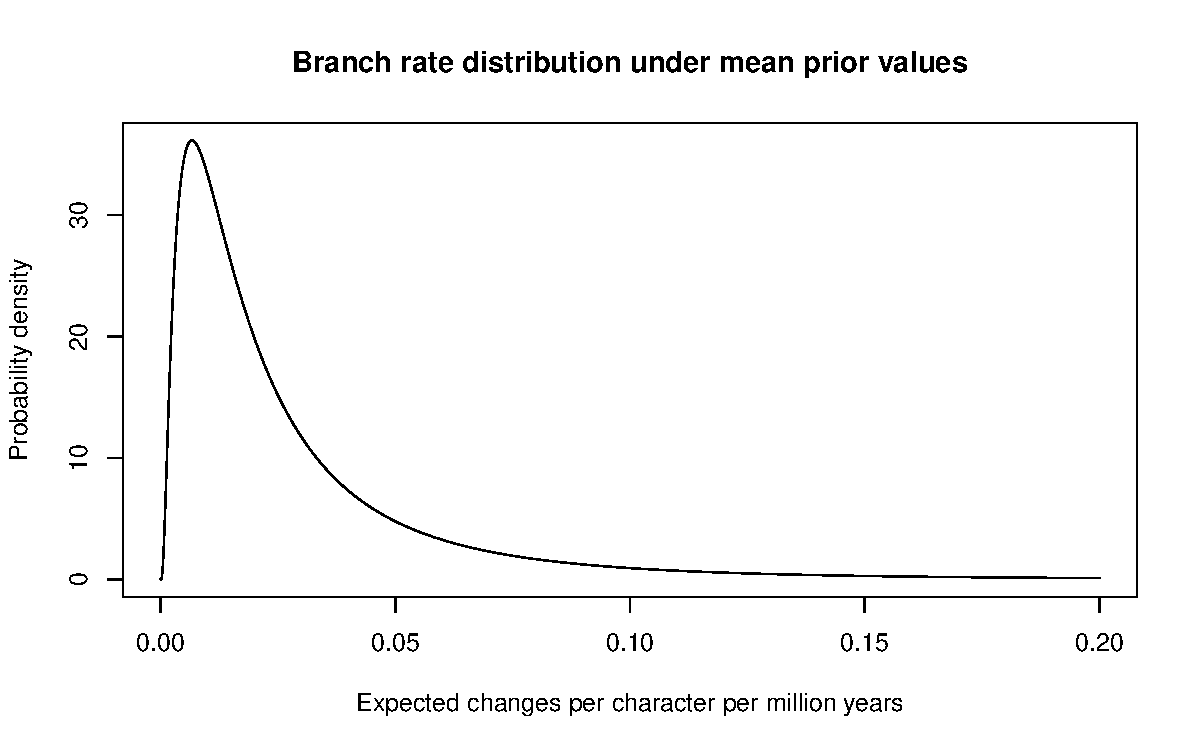
\includegraphics[width=\textwidth]{branchrateprior.pdf}

\noindent Note, however, that the actual distribution may be very different, because both parameters are in fact estimated from the data, which will presumably cause them to deviate from the prior. \\

\noindent Finally, we just need to change our call to the \texttt{dnPhyloCTMC()} function one more time: \\

\indent \texttt{characters[j] {\footnotesize $\sim$} dnPhyloCTMC(tree=tree, Q=Q[j], type="Standard",} \\
\indent \texttt{\ \ \ \ \ \ \ \ \ \ \ \ \ \ \ \ \ \ \ \ \ \ \ \ \ \ \ \ \ \ \ \ \ \ \ siteRates=char\_rates, coding="variable"} \\
\indent \texttt{\ \ \ \ \ \ \ \ \ \ \ \ \ \ \ \ \ \ \ \ \ \ \ \ \ \ \ \ \ \ \ \ \ \ \ branchRates=branch\_rates)}

\vfill

\hrule
\ \\[1ex]
\textbf{6) Repeat your analysis using the uncorrelated lognormal relaxed clock instead of the strict clock. Did the change have any impact on the topology of your tree or on your divergence time estimates?} \\

\noindent \textbf{7) Describe the posterior distributions you obtained for \texttt{ucln\_mean} and \texttt{ucln\_sigma}. What does this tell you about the branch rates for your pasta dataset? Is there a lot of variation, or are they tightly concentrated about a particular value? Based on your answer, do you think it was important to switch from the strict clock to a relaxed clock for your dataset?} \\
\hrule

\newpage

\noindent You may have noticed there is one ingredient that's missing from today's analyses, compared to the one we ran last week: nowhere in our script did we specify an outgroup. This is because we are working with rooted trees, and estimating the position of the root is part of the inference process. That's a bit of a mixed blessing: on the one hand, we can actually \textit{test} whether our outgroup forms the sister group to all other taxa in our tree, instead of just assuming it. On the other hand, our datasets are so small that they might not contain enough information to reliably infer the position of the root all on their own. \\

\hrule
\ \\[1ex]
\textbf{8) Was your analysis able to identify Orzo as the sister group of all other pastas on its own? If not, where exactly did Orzo end up in your tree?} \\
\hrule
\ \\[1ex]
\noindent We've established that we don't \textit{need} an outgroup when estimating time trees -- but \textit{could} we still specify one if we really wanted to? Of course! We can use \textit{topological constraints}, which tell RevBayes to only explore those trees that satisfy certain conditions. In particular, clade constraints require that specified taxa always form a monophyletic group to the exclusion of all the other taxa. For example, this is how we could enforce a sister-group relationship between the gray wolf (\textit{Canis lupus}) and the dire wolf (\textit{Canis dirus}): \\

\indent \texttt{tree\_distribution = dnFBDP(origin=origin\_time, lambda=speciation, rho=rho,} \\
\indent \texttt{\ \ \ \ \ \ \ \ \ \ \ \ \ \ \ \ \ \ \ \ \ \ \ \ \ \ \ \ \ \ \ \ \ mu=extinction, psi=recovery, taxa=taxa)} \\
\indent \texttt{clade\_constraints[1] = clade("Canis\_dirus", "Canis\_lupus")} \\
\indent \texttt{tree {\footnotesize $\sim$} dnConstrainedTopology(treeDistribution=tree\_distribution,} \\
\indent \texttt{\ \ \ \,\ \ \ \ \ \ \ \ \ \ \ \ \ \ \ \ \ \ \ \ \ \ \ \ \ \ \ \ \ \ \ \,\,\ constraints=clade\_constraints)} \\

\noindent What we really want is to enforce a clade that contains all taxa other than Hesperocyoninae, our former outgroup. While we could list all the 38 ingroup taxa by their names, one by one, just like we did above, that would be a pretty laborious and error-prone process. Instead, we can do the following: \\

\indent \texttt{\# Create a temporary copy of the "taxa" vector} \\
\indent \texttt{my\_taxa <- taxa} \\
\ \\
\indent \texttt{\# Remove Hesperocyoninae from the copy} \\
\indent \texttt{my\_taxa.erase(taxon("Hesperocyoninae"))} \\
\ \\
\indent \texttt{\# Set up the corresponding clade constraint} \\
\indent \texttt{my\_constraints[1] = clade(my\_taxa)} \\
\indent \texttt{tree {\footnotesize $\sim$} dnConstrainedTopology(treeDistribution=tree\_distribution,} \\
\indent \texttt{\ \ \ \,\ \ \ \ \ \ \ \ \ \ \ \ \ \ \ \ \ \ \ \ \ \ \ \ \ \ \ \ \ \ \ \,\,\ constraints=my\_constraints)} \\

\hrule
\ \\[1ex]
\textbf{9) Re-run your analysis under a topological constraint that enforces the monophyly of all non-Orzo pastas. Did the results change in any way?} \\
\hrule
\ \\[1ex]
\noindent However, maybe it's not such a good idea to include outgroups in our analysis in the first place, regardless of whether they are treated as such. Above, we've seen that the parameters of the FBD model include the fossil recovery rate ($\psi$) and extant sampling probability ($\rho$). Unfortunately, these are pretty sensitive to the fact that when researchers assemble their character matrices, they never sample the outgroup as densely as the ingroup. For example, if we use a single derived representative of a diverse clade as our outgroup, this outgroup will end up sitting at the end of a branch of very long duration. This implies a long period during which the outgroup lineage failed to leave behind any fossils, which will in turn lead the analysis to underestimate the fossil recovery rate. Only by sampling the outgroup clade more densely could we break up that long branch and get a more accurate estimate of $\psi$. Similarly, the inclusion of an outgroup makes it hard to meaningfully specify $\rho$. If my analysis includes 90\% of the extant species belonging to the ingroup clade, but only 0.1\% of the extant species belonging to the outgroup clade, what value should I use? Often, these problems are most easily avoided by removing the outgroup altogether. \\

\hrule
\ \\[1ex]
\textbf{10) Re-run your analysis without Orzo. Did this change the relationships among the remaining taxa? Are the posterior estimates of your \texttt{fossil\_prob} parameter any different now?} \\
\hrule
\end{document}